\documentclass[tikz,border=8pt]{standalone}
\usetikzlibrary{arrows.meta,calc,decorations.pathmorphing}

\begin{document}
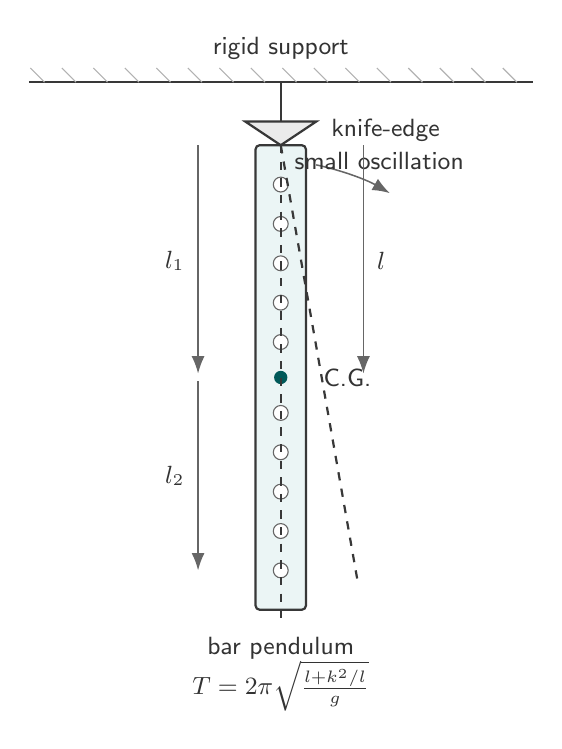
\begin{tikzpicture}[
  line/.style={line width=0.8pt, draw=black!78},
  label/.style={font=\sffamily\small, text=black!80},
  point/.style={circle, fill=teal!70!black, inner sep=1.7pt},
  hole/.style={circle, draw=black!60, fill=white, inner sep=1.9pt},
  dim/.style={-{Latex[length=2.2mm]}, line width=0.55pt, draw=black!60},
]

% Support
\draw[line, rounded corners=1pt] (-3.2,3.75) -- (3.2,3.75);
\foreach \x in {-3.0,-2.6,...,3.0} {
  \draw[black!30] (\x,3.75) -- ++(-0.18,0.18);
}
\draw[line] (0,3.75) -- (0,3.25);
\draw[line, fill=black!8] (-0.45,3.25) -- (0.45,3.25) -- (0,2.95) -- cycle;
\node[label, above] at (0,3.92) {rigid support};
\node[label, right] at (0.52,3.14) {knife-edge};

% Bar
\draw[line, fill=teal!8, rounded corners=1.5pt] (-0.32,2.95) rectangle (0.32,-2.95);
\foreach \y in {2.45,1.95,1.45,0.95,0.45,-0.45,-0.95,-1.45,-1.95,-2.45} {
  \node[hole] at (0,\y) {};
}
\node[point] at (0,0) {};
\node[label, right] at (0.42,0) {C.G.};
\node[label, below] at (0,-3.18) {bar pendulum};

% Oscillation arc
\draw[dim] (0.45,2.7) arc[start angle=78,end angle=60,radius=3.2];
\node[label] at (1.25,2.75) {small oscillation};
\draw[line, dashed] (0,2.95) -- (0,-3.05);
\draw[line, dashed, rotate around={10:(0,2.95)}] (0,2.95) -- (0,-2.7);

% Distances
\draw[dim] (-1.05,2.95) -- (-1.05,0.05);
\draw[dim] (-1.05,-0.05) -- (-1.05,-2.45);
\node[label, left] at (-1.1,1.48) {$l_1$};
\node[label, left] at (-1.1,-1.25) {$l_2$};

\draw[dim] (1.05,2.95) -- (1.05,0.05);
\node[label, right] at (1.1,1.48) {$l$};

\node[label, align=center] at (0,-3.92)
  {$T=2\pi\sqrt{\frac{l+k^2/l}{g}}$};

\end{tikzpicture}
\end{document}
